%\begin{frame}
%\frametitle{Massive neutrinos}
%\begin{columns}
%\column{0.4\textwidth}
%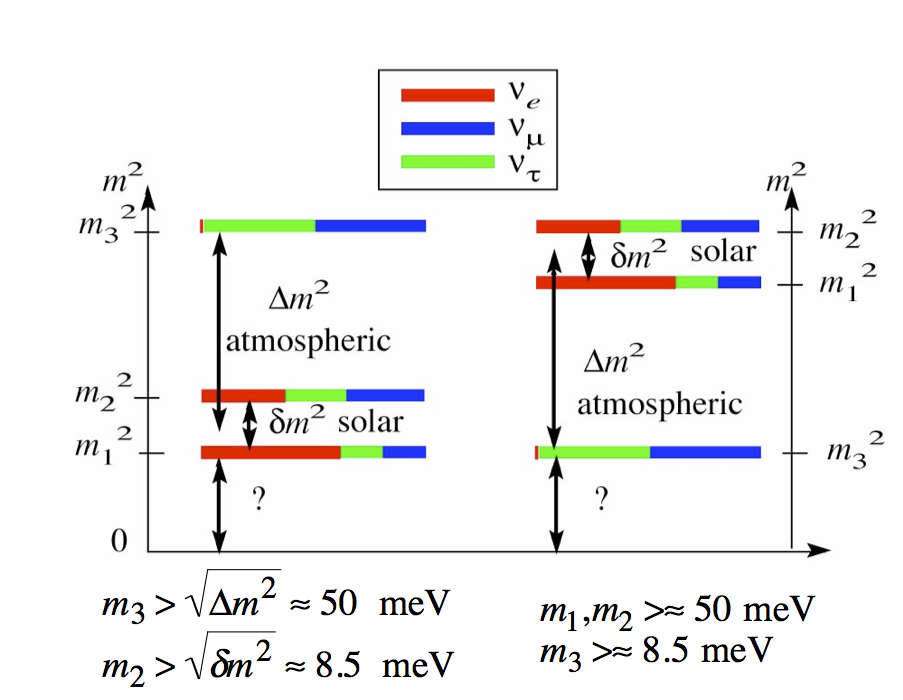
\includegraphics[scale=0.35]{MassNeutrinos.png}
% 
% \column{0.5\textwidth}
%%\begin{block}{}
%Neutrino oscillation experiments (a story to be told some other time) have established that neutrinos are massive. Their mass is, however, very small. This is the reason why parity experiments found the neutrino to be left handed, since the effects associated to their masses are of the order of $m/E$~where $m$~is the mass of the neutrino (tiny) and $E$~the energy of the process (much larger). 
%
%\alert{But how do we give a mass to the neutrinos?} 
%
%%\end{block}
%\end{columns}
%\end{frame}

%\begin{frame}
%\frametitle{Electron mass}
%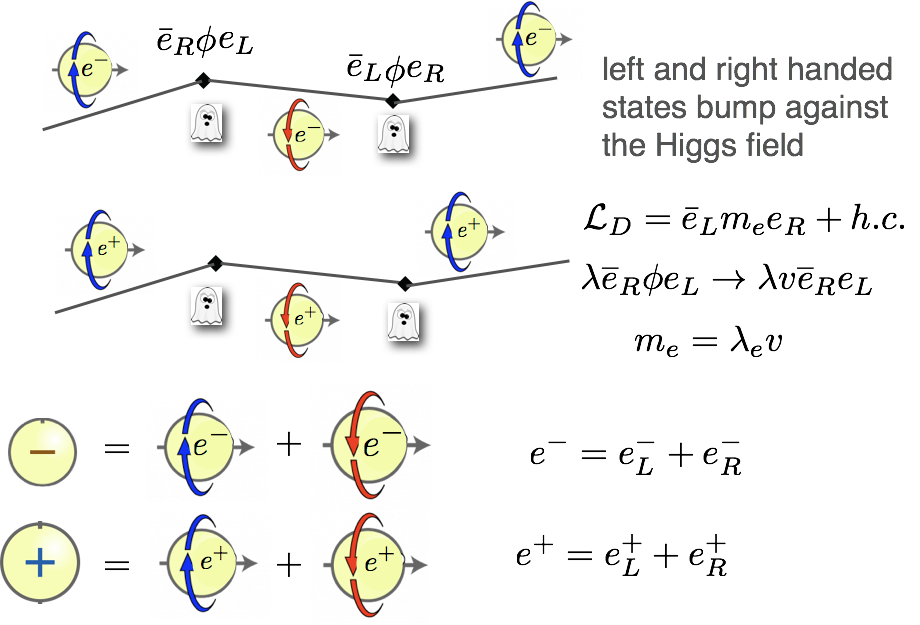
\includegraphics[scale=0.30]{ElectronMass.png}
%\end{frame}
%
%\begin{frame}
%\frametitle{Neutrino mass (Dirac recipe)}
%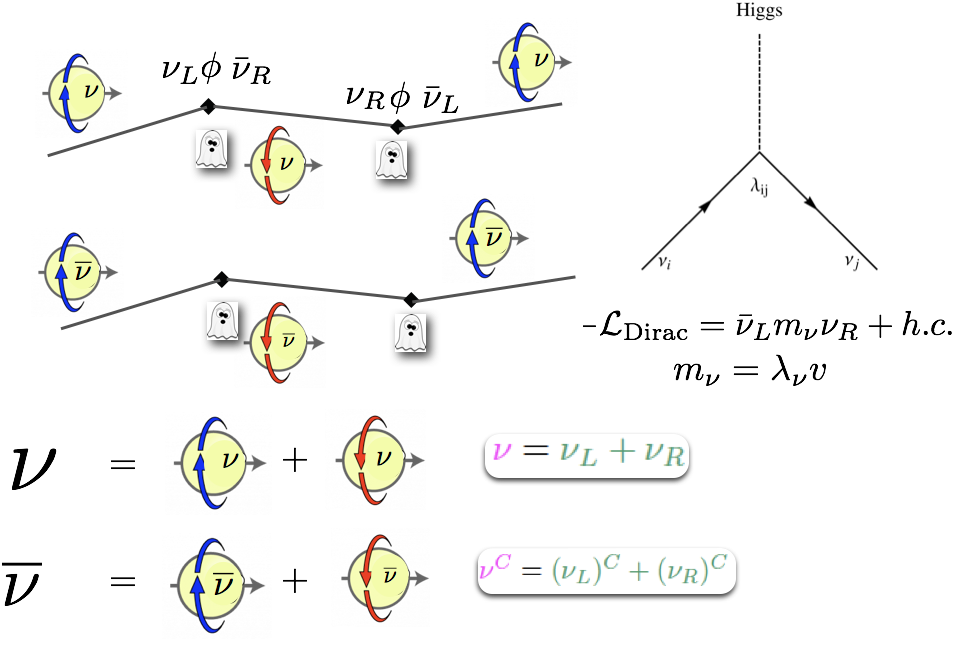
\includegraphics[scale=0.30]{NeutrinoMassDirac.png}
%\end{frame}

%\begin{frame}
%\frametitle{Deus ex machina}
%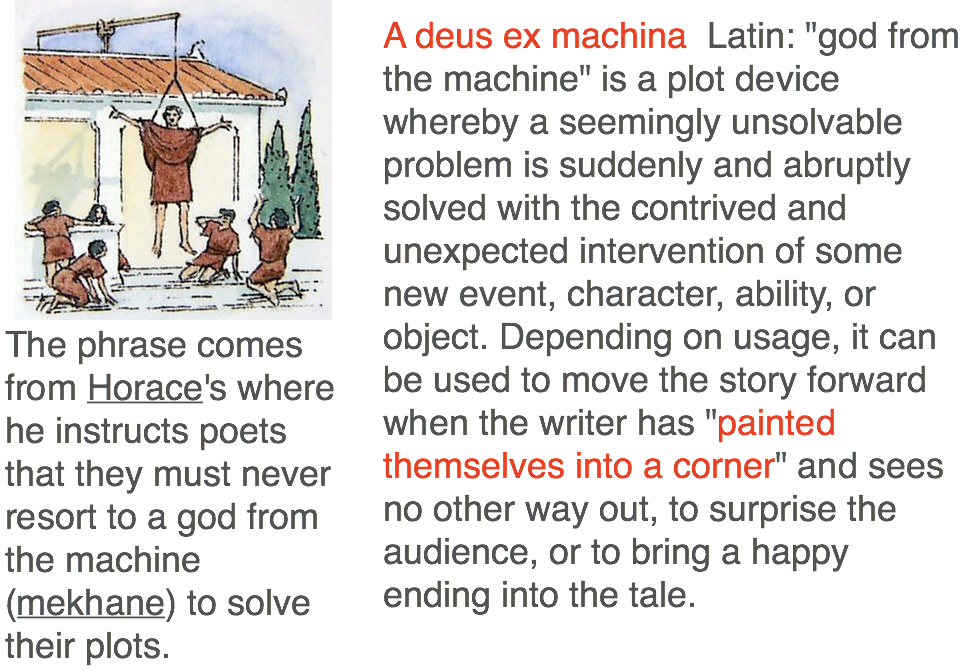
\includegraphics[scale=0.30]{DeusExMachina.png}
%\end{frame}
%
%\begin{frame}
%\frametitle{Dirac neutrino mass: Deus ex machina}
%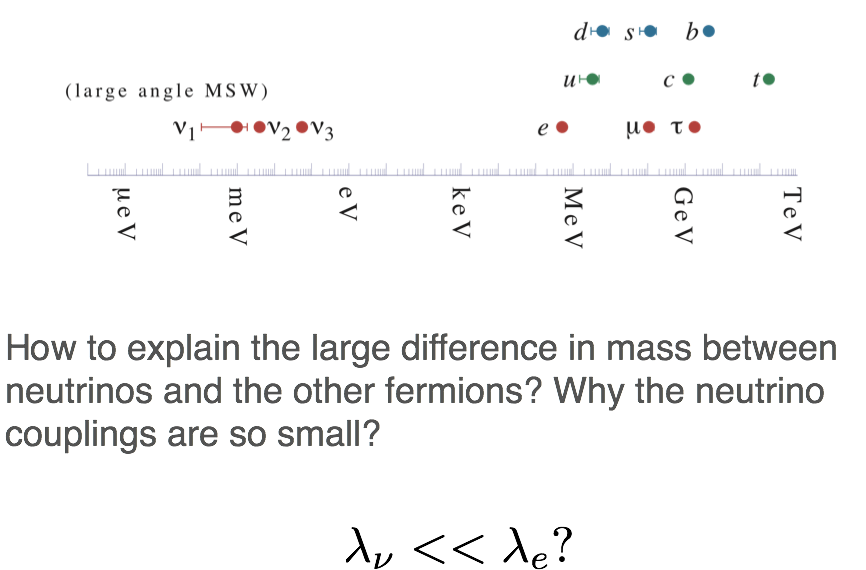
\includegraphics[scale=0.30]{SmallNeutrinoMasses.png}
%\end{frame}

%\begin{frame}
%\frametitle{Majorana neutrinos}
%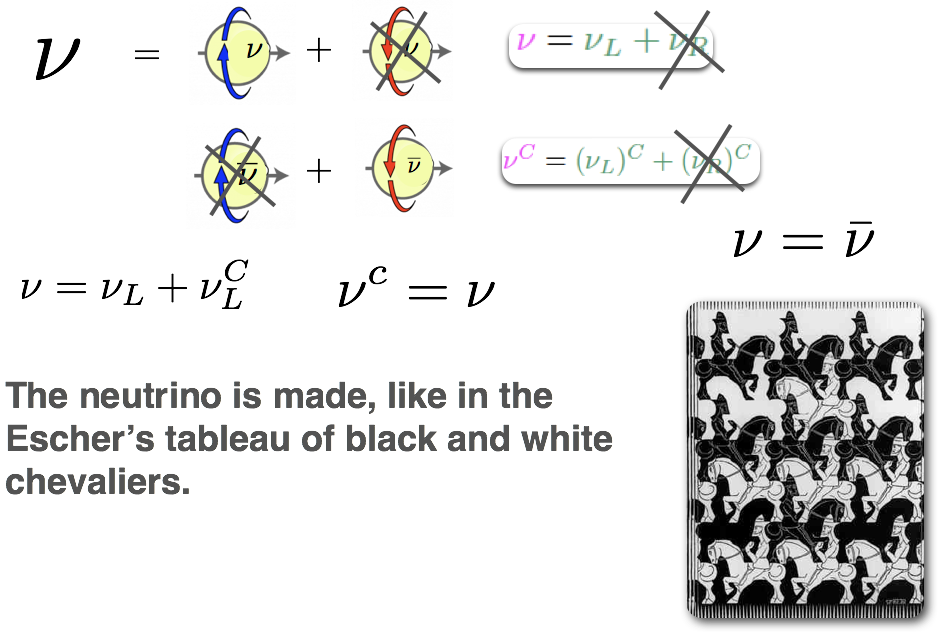
\includegraphics[scale=0.30]{MajoranaNeutrinosCartoon.png}
%\end{frame}
%
%\begin{frame}
%\frametitle{Majorana mass}
%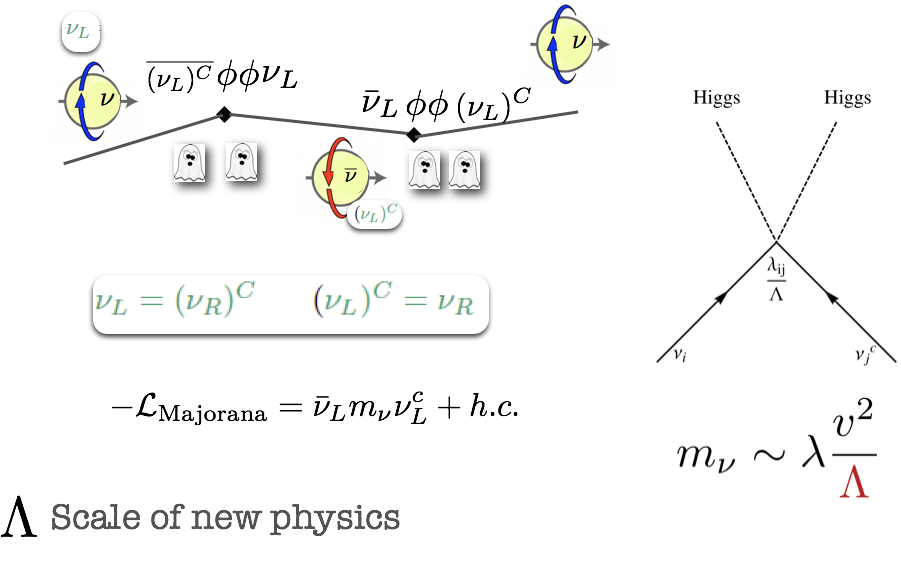
\includegraphics[scale=0.30]{MajoranaMass.png}
%\end{frame}
%
%\begin{frame}
%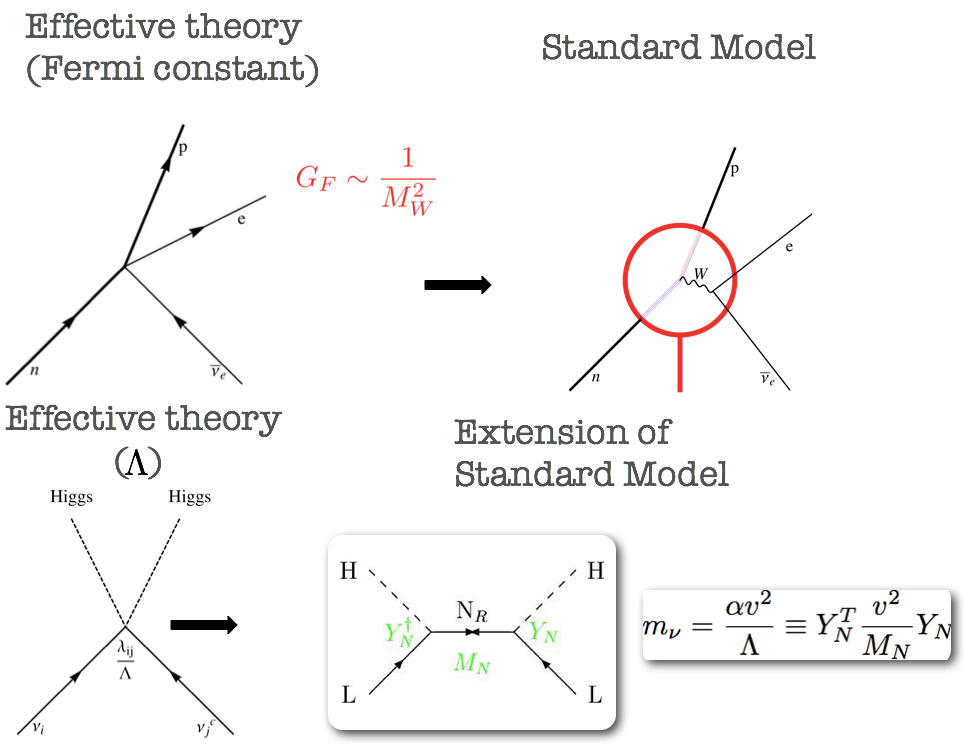
\includegraphics[scale=0.30]{Effective.png}
%\end{frame}

\begin{frame}
\frametitle{The mystery of the missing antimatter}
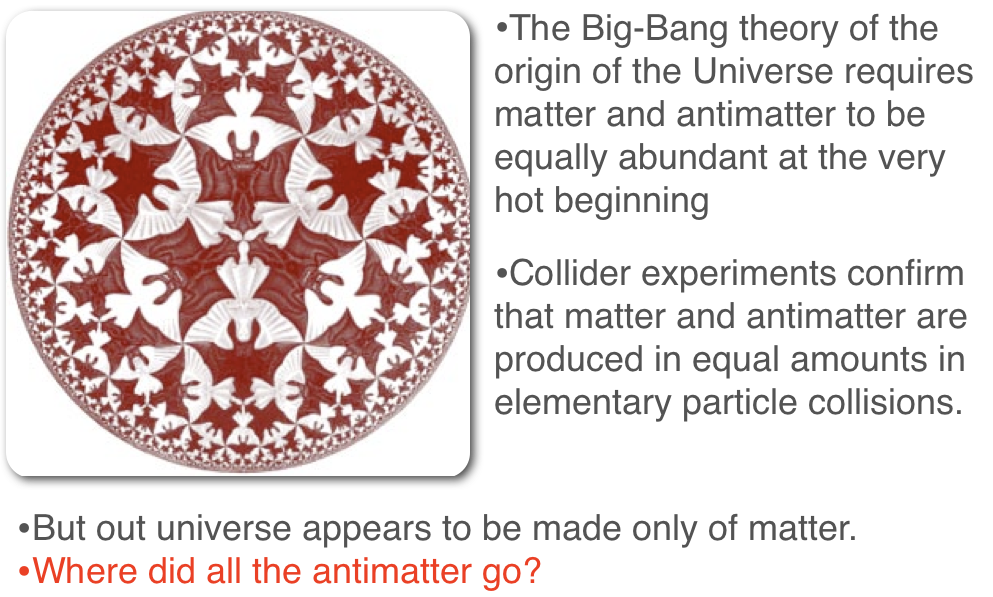
\includegraphics[scale=0.30]{MissingAntiMatter.png}
\end{frame}

\begin{frame}
\frametitle{CP violation and Majorana neutrinos}
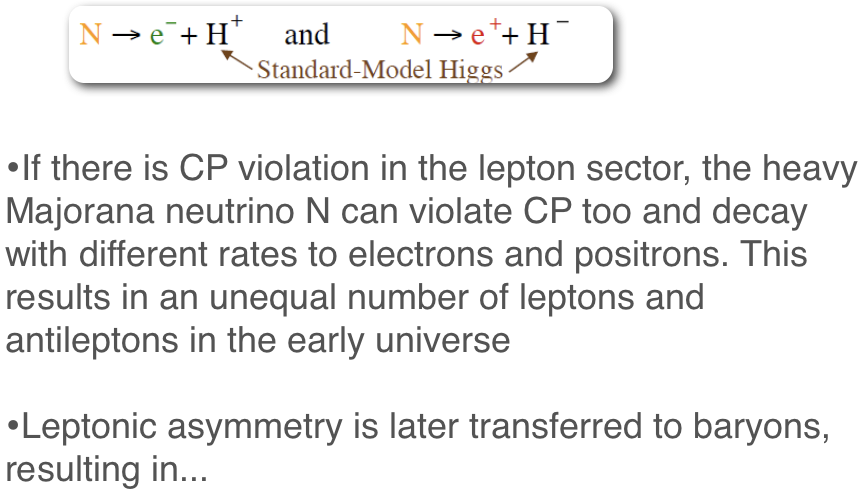
\includegraphics[scale=0.30]{CP.png}
\end{frame}

\begin{frame}
\frametitle{We are the leftovers}
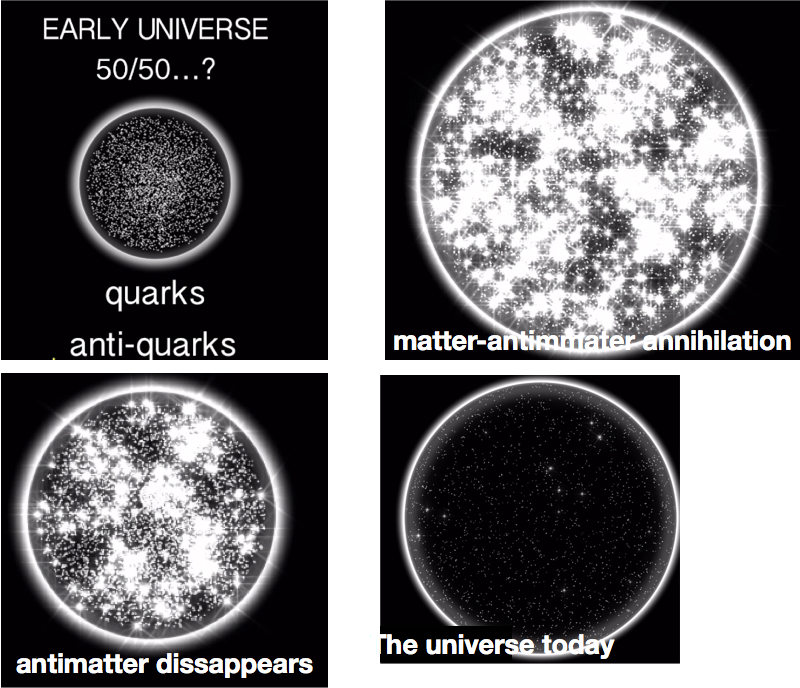
\includegraphics[scale=0.30]{MissingUniverse.png}
\end{frame}

\begin{frame}
\frametitle{Are neutrinos Majorana Particles?}

\includegraphics[scale=0.30]{DoubleOrNothing.png}
\end{frame}

\begin{frame}
\frametitle{Double Beta Decay}
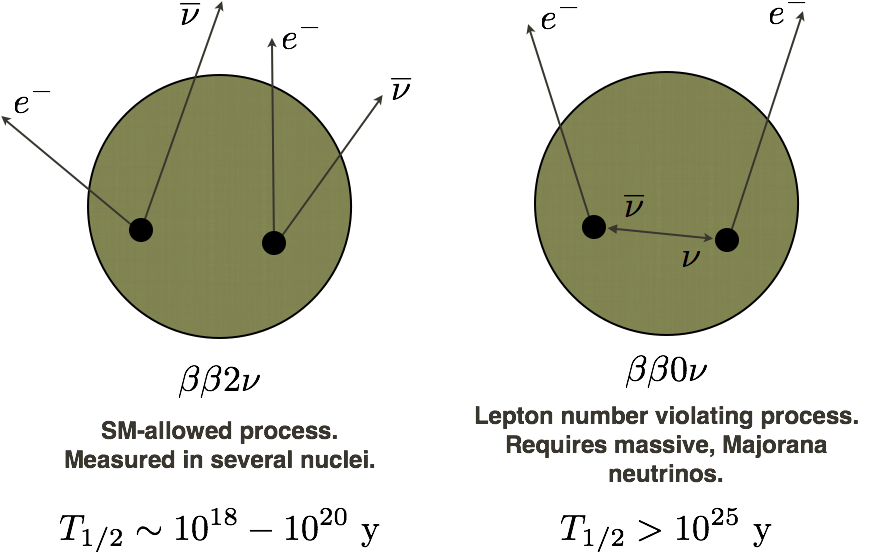
\includegraphics[scale=0.30]{DoubleBetaDecay.png}
\end{frame}

\begin{frame}
\frametitle{Double Beta Decay}
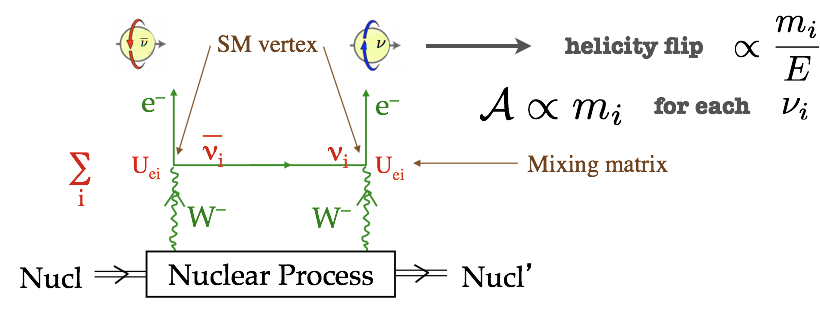
\includegraphics[scale=0.20]{DoubleBetaDiagram2.png}

%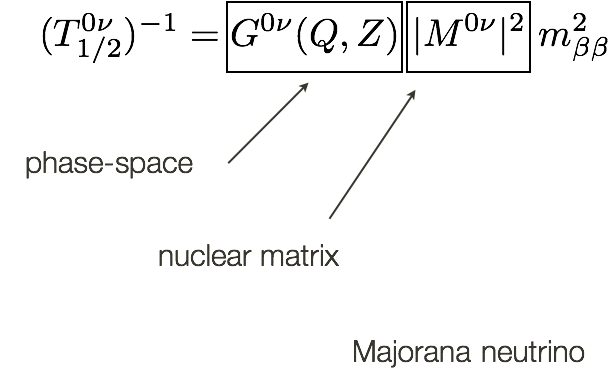
\includegraphics[scale=0.30]{DoubleBetaLifetime.png}
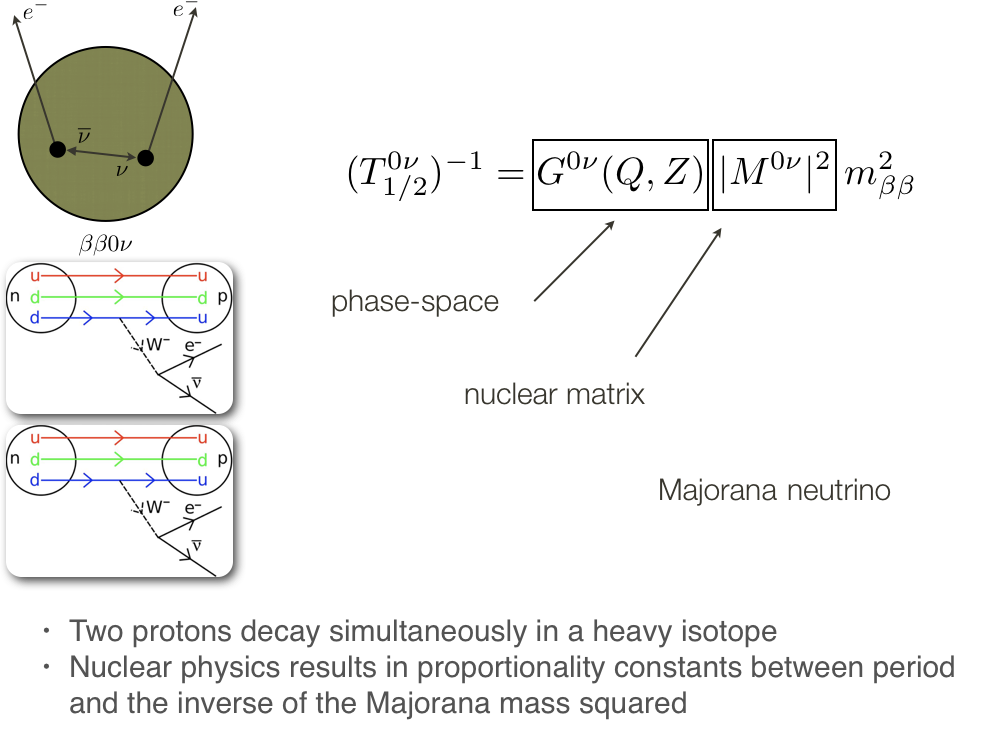
\includegraphics[scale=0.20]{bbmatrix.png}


\end{frame}



\begin{frame}
\frametitle{An Ideal double beta decay experiment}
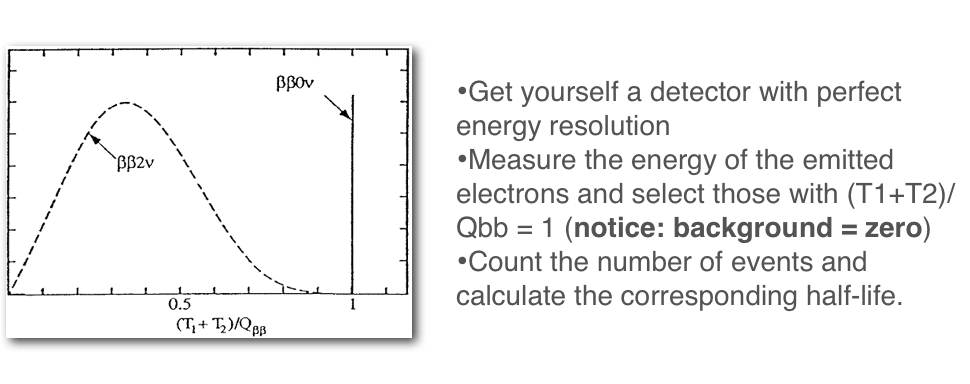
\includegraphics[scale=0.30]{IdealBB.png}
\end{frame}

\begin{frame}
\frametitle{How difficult is to observe $\beta\beta0\nu$~decays}
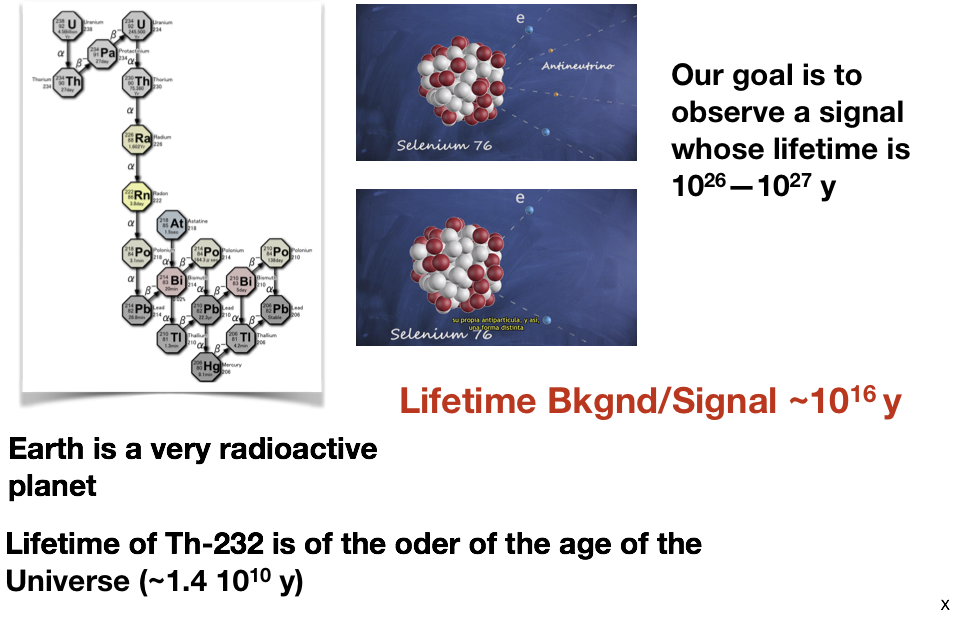
\includegraphics[scale=0.30]{RadioactiveEarth.png}
\end{frame}

\begin{frame}
\frametitle{Majorana Beach}
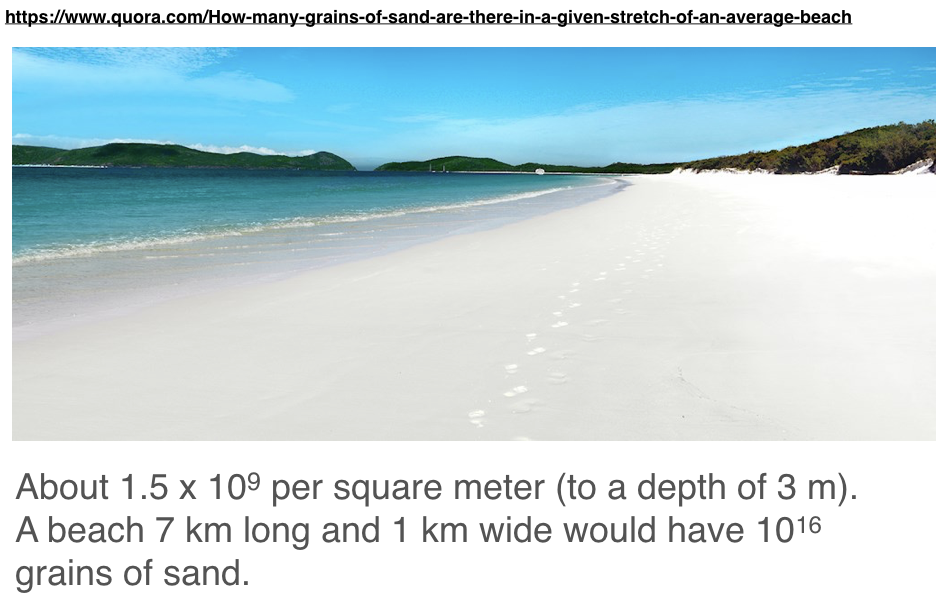
\includegraphics[scale=0.30]{MajoranaBeach.png}
\end{frame}

\begin{frame}
\frametitle{The NEXT experiment at the LSC}
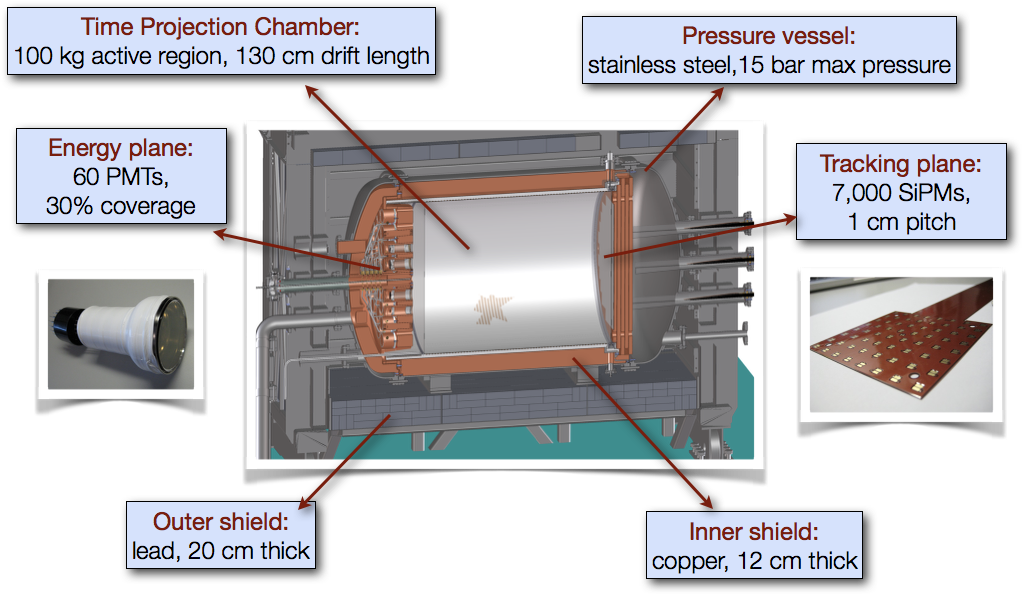
\includegraphics[scale=0.30]{Next100.png}
\end{frame}

\begin{frame}
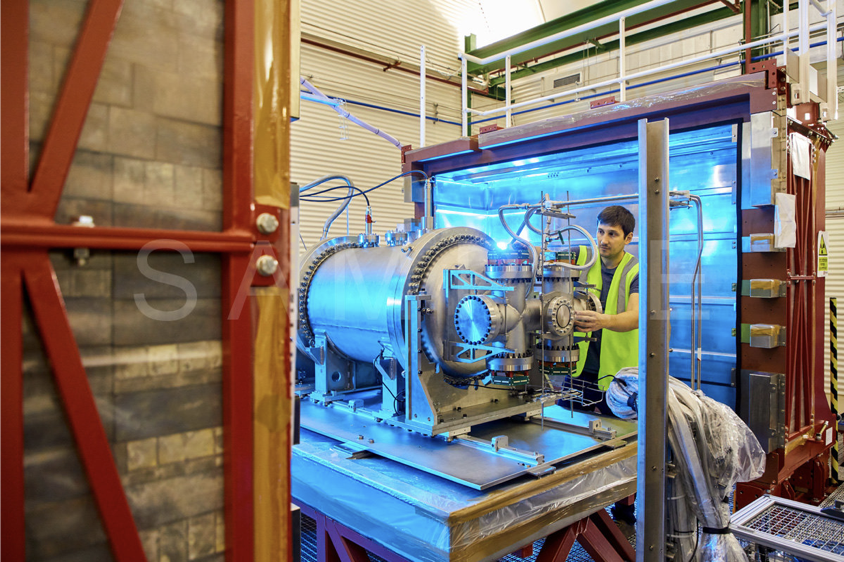
\includegraphics[scale=0.30]{NEW.png}
\end{frame}

\begin{frame}
\frametitle{Majorana Beach}
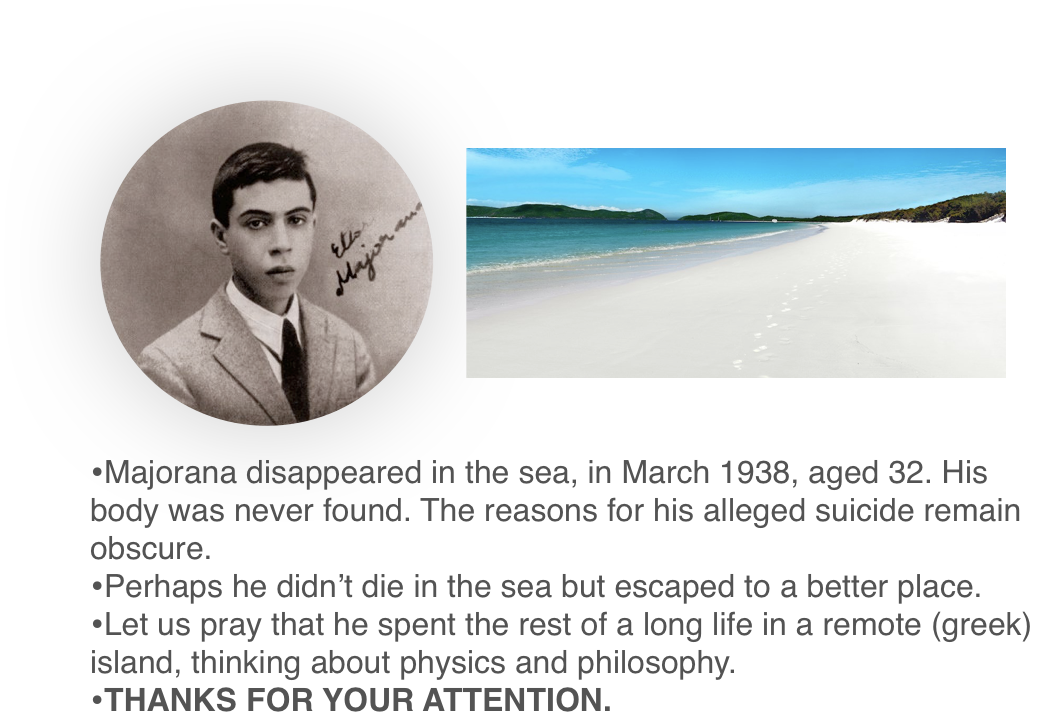
\includegraphics[scale=0.30]{MajoranaBeach2.png}
\end{frame}















